%
% File naaclhlt2010.tex
%
% Contact: nasmith@cs.cmu.edu

\documentclass[11pt,letterpaper]{article}
\usepackage{naaclhlt2010}
\usepackage{times}
\usepackage{latexsym}
\usepackage{graphicx}
\setlength\titlebox{6.5cm}    % Expanding the titlebox

\title{Optimization of Nearest Neighbors: Run Time and Accuracy}

\author{Kyle Wong \\
  3400 N. Charles St. \\
  Baltimore, MD 21218 \\
  {\tt kwong23@jhu.edu}
  \And
  Tifany Yung \\
  3400 N. Charles St. \\
  Baltimore, MD 21218 \\
  {\tt tyung1@jhu.edu}}

\date{May 12, 2014}

\begin{document}
\maketitle
\begin{abstract}
Ligands can react with a particular receptor in one of three ways: bind and activate the receptor, bind and inhibit the receptor, and not bind at all. Whether a ligand is likely to bind to a receptor can be determined by considering the features such as ligand and receptor shapes, charges, and molecular forces. All of the factors can be accounted via FRED (Fast Rigid Exhaustive Docking) which calculates the Chemgauss4 (cg4) scoring function.

Since the relative positions of both the ligand and receptor affect the likelihood of binding, the FRED scores for 500 receptor frames crossed with each of 710 ligands were taken to create a system for predicting whether a particular ligand will bind with the receptor. These 500 frames were used as the features for feature vectors with the ligands as an instances.

The labeled ligand instances and their 500-FRED-score-long feature vectors were used to train a basic $\epsilon$-sphere, nearest neighbors algorithm with low precision and recall results. The algorithm was then improved by selecting features with information gain and testing with different $\epsilon$ values.  However, the original dataset proved to be too small and limited to get conclusive results.  Synthetic data was then generated for testing and improving the nearest neighbors algorithm.  Then, the nearest neighbors algorithm was improved using a Lamba Means EM (Expectation Maximization) algorithm to cluster the data points with highly positive results.  
\end{abstract}

\section{Introduction}
\subsection{Nearest Neighbor Algorithm}

The $\epsilon$-sphere nearest neighbors algorithm is a close relative of the K-nearest neighbors algorithm; both are clustering algorithms designed with the purpose of categorizing data into a certain number of categories, or labels. As an example, for the ligand-receptor data used, the ligands would be labeled with whether or not they bind with the given receptor.

Clustering algorithms work by using nearby points to determine which cluster or label a given point should be placed in based on the labels of the points around it. The only difference between the above-mentioned $\epsilon$-sphere and K nearest neighbors is how to choose the points around the test point to help determine the test point's label. In the K nearest neighbors algorithm, the number K of points closest to the test point are taken, and the test point is assigned the majority label amongst those points; in the $\epsilon$-sphere algorithm, all points that are within a Euclidean distance of $\epsilon$ or less from the test point are used and the majority label is used as the prediction.

The general structure of the $\epsilon$-sphere clustering algorithm is the same as any machine learning algorithm: teaching the algorithm using a training dataset, and testing the accuracy of the algorithm with a development dataset. During training of $\epsilon$-sphere clustering, the training data points are simply read in and stored. 

During testing, data points are input individually, and the algorithm attempts to predict their label. It does so by taking all data points within Euclidean distance $\epsilon$ of the test point and calculating the majority label amongst those points. The test point is then assigned to that majority label.

There has been some previous research into speeding up K nearest neighbors by using $\epsilon$-sphere. Indyk and Rajeev (1998) first implemented and tested a kd-tree for the $\epsilon$-sphere algorithm and recommended it only for low-dimensional data. More recently, Muja and Lowe attempted to find fast approximates for the nearest neighbors algorithm.

\subsection{Virtual Screening}
For receptor ligand docking, much of the work is done manually by hand where researchers do virtual screening for a given receptor by hand-picking ligands that they believe will likely bind to the receptor.  This process is known to be very slow and labor-intensive.  As such, automated virtual screening is of utmost importance.  However, simply screening a receptor model with a ligand in a docking program such as FRED often results in incorrect estimates of binding affinity.  The assumption is that ligands that bind to a receptor will fit nicely with the receptor and will thus be detected by having a more negative binding score when screened with docking.  However, oftentimes, ligands that do not bind to a receptor sometimes give a more negative binding score for a given receptor pose. Thus, using multiple receptor poses may improve docking calculations (Totrov et. al. 2008).

However, receptor model poses are frequently incomplete as the conformational space of protein shape and flexibility is so large.  This leads to a wide fluctuation in binding affinity score predictions.  One approach for addressing this issue is identifying the relevant receptor modes to identify the correct ensemble of receptor conformations in order to do more accurate virtual screening (Cavasotto 2005).  This leads to the idea of applying the concept of measuring Information Gain on the receptor frame (pose) features in order to select the frames which are truly relevant.

\section{Data}
The data used for this project includes Ligand/receptor binding data obtained from the Data Management Systems lab. The data consists of 710 labeled ligands that were screened with FRED across 500 frames of a receptor to get Chemgauss4 (cg4) scores. Each receptor frame represents the pose of a receptor at a different time.  10 of the ligands were known to actively bind with the receptor while the other 700 ligands were known to not have binding activity with the receptor.

\section{Methods}
\subsection{Algorithm Selection}
For this project, we assumed that the different frames of the receptor would capture different characteristics of ligands required for the ligand to bind to the receptor.  Therefore, since we had 500 frame data points for each ligand, we chose to do the $\epsilon$-sphere nearest neighbors algorithm under the idea that if two ligands had similar binding scores for the same frames, they would be functionally similar.  Thus, they would have a low Euclidean distance in terms of the frame FRED cg4 scores.

There are a variety of characteristics that can help a ligand to bind to a receptor including: electrostatics forces, solvation and desolvation effects, hydrophobic interactions, bond stretching, dihedral energy terms, hydrogen bonds, and many other factors.  Therefore, our idea was that ligands that bound to the receptor would score similarly to other binding ligands.  And in the same way, non-binding ligands would score similarly to non-binding ligands.  So using the $\epsilon$-sphere nearest neighbors algorithm would help us to identify regions in the frame-ligand score space that corresponded to binding ligands.

\subsection{Algorithm Optimization}
Since some of the receptor frames (the features) may not provide useful and accurate information about ligand binding potential, we decided to try to use a measure of Information Gain to select the best frames for distinguishing whether a ligand would bind or not.  Since we had many frames, there was thus a high dimensionality, so reducing the number of features using Information Gain would also help overcome the "Curse of Dimensionality."  

Since the nearest neighbor algorithm requires iterating over all the training points for every single prediction, we considered creating a KD-Tree data structure to more quickly identify the nearest points.  However, upon further research we realized that KD-trees are not helpful in high-dimensional spaces.  For example, one general rule is that if the dimensionality is k, the number of points in the data, N, should be N much greater than $2^k$. If this is not the case, then a KD-tree will simply evaluate nearly all the points in the tree, and the efficiency is no better than exhaustive search (Goodman et al. 2004).  And in our case, we have $k=500$ and $N=710$ in which case using a KD-tree might even be slower than just exhaustive search.

Thus, we instead implemented a Lambda-Means approach where we would use EM (Expectation Maximization) to cluster points that were close together in terms of Euclidean distance.  Then, when predicting, we would first compare to the prototype vectors and then would only need to compare to the points within that cluster to find the majority of labels of points within the distance $\epsilon$.  In a sense, this approach would be like sorting the training points into different buckets to speed up prediction time by ignoring points that have an average distance that is further away.  This would give us a way to improve the slow runtime of the nearest neighbor algorithm which normally exhaustively must check against all of the training points while not sacrificing accuracy.


\section{Results}
The algorithm accuracy, precision, recall, and run time in milliseconds for the K-means algorithm is shown below for when all features are used and when only the fifty with the highest information gain are used.

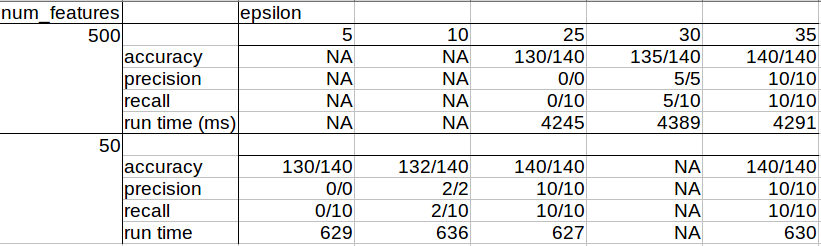
\includegraphics[width=75mm]{formattedData.png}

- what tests did we run

- what do these results mean

\section{Comparison}

The original project proposal suggested three milestones for the optimization of nearest neighbors: minimum, expected, and stretch deliverables. The minimum deliverable was to implement a functional $\epsilon$-sphere nearest neighbor algorithm to predict whether or not a ligand will potentially respond and bind to a given receptor and to implement feature selection via information gain. This implementation was achieved and presented in the class SphereNearestNeighborPredictor.java in the "sphere" package of the "neighbors" project; the results and analysis of the run time and accuracy of this implementation is provided above in the Results section.

The expected deliverable was to implement a faster $\epsilon$-sphere algorithm by using divide-and-conquer in lieu of a linear search for the $epsilon$ closest points to a test point, similar to a kd tree. However, this was not implemented because it was found via additional research (Indyk and Rajeev) that usage of kd trees in higher dimensions are no better than brute-force search since most nodes in the kd tree would need to be evaluated anyways. Therefore, this deliverable was not implemented.

Instead, the time was used to implemented 

\section{Junk}
Manuscripts must be in two-column format.  Exceptions to the
two-column format include the title, authors' names and complete
addresses, which must be centered at the top of the first page (see
the guidelines in Subsection~\ref{ssec:first}), and any full-width
figures or tables .  Type single-spaced.  Do not number the pages.
Start all pages directly under the top margin.  See the guidelines
later regarding formatting the first page.

The maximum length of a manuscript is eight (8) pages for the main
conference, printed single-sided, plus one (1) page for references
(see Section~\ref{sec:length} for additional information on the
maximum number of pages).  Do not number the pages.

\subsection{Electronically-available resources}

NAACL HLT provides this description in \LaTeX2e{} ({\tt naaclhlt2010.tex}) and PDF
format ({\tt naaclhlt2010.pdf}), along with the \LaTeX2e{} style file used to
format it ({\tt naaclhlt2010.sty}) and an ACL bibliography style ({\tt naaclhlt2010.bst}).
These files are all available at
{\tt http://naaclhlt2010.isi.edu}.  A Microsoft Word
template file ({\tt naaclhlt2010.dot}) is also available at the same URL. We
strongly recommend the use of these style files, which have been
appropriately tailored for the NAACL HLT 2010 proceedings.


\subsection{Format of Electronic Manuscript}
\label{sect:pdf}

For the production of the electronic manuscript you must use Adobe's
Portable Document Format (PDF). This format can be generated from
postscript files: on Unix systems, you can use {\tt ps2pdf} for this
purpose; under Microsoft Windows, you can use Adobe's Distiller, or
if you have cygwin installed, you can use {\tt dvipdf} or
{\tt ps2pdf}.  Note 
that some word processing programs generate PDF which may not include
all the necessary fonts (esp. tree diagrams, symbols). When you print
or create the PDF file, there is usually an option in your printer
setup to include none, all or just non-standard fonts.  Please make
sure that you select the option of including ALL the fonts.  {\em
  Before sending it, test your {\/\em PDF} by printing it from a
  computer different from the one where it was created}. Moreover,
some word processor may generate very large postscript/PDF files,
where each page is rendered as an image. Such images may reproduce
poorly.  In this case, try alternative ways to obtain the postscript
and/or PDF.  One way on some systems is to install a driver for a
postscript printer, send your document to the printer specifying
``Output to a file'', then convert the file to PDF.

For reasons of uniformity, Adobe's {\bf Times Roman} font should be
used. In \LaTeX2e{} this is accomplished by putting

\begin{quote}
\begin{verbatim}
\usepackage{times}
\usepackage{latexsym}
\end{verbatim}
\end{quote}
in the preamble.

Additionally, it is of utmost importance to specify the {\bf
  US-Letter format} (8.5in $\times$ 11in) when formatting the paper.
When working with {\tt dvips}, for instance, one should specify {\tt
  -t letter}.

Print-outs of the PDF file on US-Letter paper should be identical to the
hardcopy version.  If you cannot meet the above requirements about the
production of your electronic submission, please contact the
publication chairs above  as soon as possible.


\subsection{Layout}
\label{ssec:layout}

Format manuscripts two columns to a page, in the manner these
instructions are formatted. The exact dimensions for a page on US-letter
paper are:

\begin{itemize}
\item Left and right margins: 1in
\item Top margin:1in
\item Bottom margin: 1in
\item Column width: 3.15in
\item Column height: 9in
\item Gap between columns: 0.2in
\end{itemize}

\noindent Papers should not be submitted on any other paper size. Exceptionally,
authors for whom it is \emph{impossible} to format on US-Letter paper,
may format for \emph{A4} paper. In this case, they should keep the \emph{top}
and \emph{left} margins as given above, use the same column width,
height and gap, and modify the bottom and right margins as necessary.
Note that the text will no longer be centered.

\subsection{The First Page}
\label{ssec:first}

Center the title, author's name(s) and affiliation(s) across both
columns. Do not use footnotes for affiliations.  Do not include the
paper ID number assigned during the submission process. 
Use the two-column format only when you begin the abstract.

{\bf Title}: Place the title centered at the top of the first page, in
a 15 point bold font.  (For a complete guide to font sizes and styles, see Table~\ref{font-table}.)
Long title should be typed on two lines without
a blank line intervening. Approximately, put the title at 1in from the
top of the page, followed by a blank line, then the author's names(s),
and the affiliation on the following line.  Do not use only initials
for given names (middle initials are allowed). Do not format surnames
in all capitals (e.g., ``Leacock,'' not ``LEACOCK'').  The affiliation should
contain the author's complete address, and if possible an electronic
mail address. Leave about 0.75in between the affiliation and the body
of the first page.

{\bf Abstract}: Type the abstract at the beginning of the first
column.  The width of the abstract text should be smaller than the
width of the columns for the text in the body of the paper by about
0.25in on each side.  Center the word {\bf Abstract} in a 12 point
bold font above the body of the abstract. The abstract should be a
concise summary of the general thesis and conclusions of the paper.
It should be no longer than 200 words.  The abstract text should be in 10 point font.

{\bf Text}: Begin typing the main body of the text immediately after
the abstract, observing the two-column format as shown in 
the present document.  Do not include page numbers.

{\bf Indent} when starting a new paragraph. For reasons of uniformity,
use Adobe's {\bf Times Roman} fonts, with 11 points for text and 
subsection headings, 12 points for section headings and 15 points for
the title.  If Times Roman is unavailable, use {\bf Computer Modern
  Roman} (\LaTeX2e{}'s default; see section \ref{sect:pdf} above).
Note that the latter is about 10\% less dense than Adobe's Times Roman
font.

\subsection{Sections}

{\bf Headings}: Type and label section and subsection headings in the
style shown on the present document.  Use numbered sections (Arabic
numerals) in order to facilitate cross references. Number subsections
with the section number and the subsection number separated by a dot,
in Arabic numerals. 

{\bf Citations}: Citations within the text appear
in parentheses as~\cite{Gusfield:97} or, if the author's name appears in
the text itself, as Gusfield~\shortcite{Gusfield:97}. 
Append lowercase letters to the year in cases of ambiguities.  
Treat double authors as in~\cite{Aho:72}, but write as 
in~\cite{Chandra:81} when more than two authors are involved. 
Collapse multiple citations as in~\cite{Gusfield:97,Aho:72}.

\textbf{References}: Gather the full set of references together under
the heading {\bf References}; place the section before any Appendices,
unless they contain references. Arrange the references alphabetically
by first author, rather than by order of occurrence in the text.
Provide as complete a citation as possible, using a consistent format,
such as the one for {\em Computational Linguistics\/} or the one in the 
{\em Publication Manual of the American 
Psychological Association\/}~\cite{APA:83}.  Use of full names for
authors rather than initials is preferred.  A list of abbreviations
for common computer science journals can be found in the ACM 
{\em Computing Reviews\/}~\cite{ACM:83}.

The \LaTeX{} and Bib\TeX{} style files provided roughly fit the
American Psychological Association format, allowing regular citations, 
short citations and multiple citations as described above.

{\bf Appendices}: Appendices, if any, directly follow the text and the
references (but see above).  Letter them in sequence and provide an
informative title: {\bf Appendix A. Title of Appendix}.

\textbf{Acknowledgment} sections should go as a last (unnumbered) section immediately
before the references.  

\subsection{Footnotes}

{\bf Footnotes}: Put footnotes at the bottom of the page. They may
be numbered or referred to by asterisks or other
symbols.\footnote{This is how a footnote should appear.} Footnotes
should be separated from the text by a line.\footnote{Note the
line separating the footnotes from the text.}  Footnotes should be in 9 point font.

\subsection{Graphics}

{\bf Illustrations}: Place figures, tables, and photographs in the
paper near where they are first discussed, rather than at the end, if
possible.  Wide illustrations may run across both columns and should be placed at
the top of a page. Color illustrations are discouraged, unless you have verified that 
they will be understandable when printed in black ink.

\begin{table}
\begin{center}
\begin{tabular}{|l|rl|}
\hline \bf Type of Text & \bf Font Size & \bf Style \\ \hline
paper title & 15 pt & bold \\
author names & 12 pt & bold \\
author affiliation & 12 pt & \\
the word ``Abstract'' & 12 pt & bold \\
section titles & 12 pt & bold \\
document text & 11 pt  &\\
abstract text & 10 pt & \\
captions & 10 pt & \\
bibliography & 10 pt & \\
footnotes & 9 pt & \\
\hline
\end{tabular}
\end{center}
\caption{\label{font-table} Font guide. }
\end{table}

{\bf Captions}: Provide a caption for every illustration; number each one
sequentially in the form:  ``Figure 1. Caption of the Figure.'' ``Table 1.
Caption of the Table.''  Type the captions of the figures and 
tables below the body, using 10 point text.  

\section{Length of Submission}
\label{sec:length}

The NAACL HLT 2010 main conference accepts submissions of long papers
and short papers.  The maximum length of a long paper manuscript is
eight (8) pages of content and one (1) additional page of references
\emph{only} (appendices count against the eight pages, not the
additional one page).  The maximum length of a short paper manuscript
is four (4) pages including references.  For both long and short
papers, all illustrations, references, and appendices must be
accommodated within these page limits, observing the formatting
instructions given in the present document.  Papers that do not
conform to the specified length and formatting requirements are
subject to be rejected without review.


\begin{thebibliography}{}
\bibitem[\protect\citename{Cavasotto, Claudio N., Julio A. Kovacs, and Ruben A. Abagyan.}2005] {Cavasotto, Claudio N., Julio A. Kovacs, and Ruben A. Abagyan.: 05} Cavasotto, Claudio N., Julio A. Kovacs, and Ruben A. Abagyan.
\newblock Representing receptor flexibility in ligand docking through relevant normal modes.
\newblock {\em Journal of the American Chemical Society}, 127.26 (2005): 9632-9640.

\bibitem[\protect\citename{Cover, Thomas, and Peter Hart.}1967]{Cover, Thomas, and Peter Hart: 67} Cover, Thomas, and Peter Hart.
\newblock 1967.
\newblock Nearest neighbor pattern classification.
\newblock {\em Information Theory, IEEE Transactions}, 13(1):21-27.

\bibitem[\protect\citename{Fukunaga, Keinosuke, and Patrenahalli M. Narendra.}1975] {Fukunaga, Keinosuke, and Patrenahalli M. Narendra: 75} Fukunaga, Keinosuke, and Patrenahalli M. Narendra.
\newblock 1975.
\newblock A branch and bound algorithm for computing k-nearest neighbors.
\newblock {\em Computers, IEEE Transactions}, 100(7): 750-753.

\bibitem[\protect\citename{Goodman, Jacob E., and Joseph O'Rourke.}2004]{Goodman, Jacob E., and Joseph O'Rourke: 04} Goodman, Jacob E., and Joseph O'Rourke.
\newblock 2004.
\newblock Handbook of discrete and computational geometry.
\newblock {\em CRC press}, 2004.

\bibitem[\protect\citename{Indyk, Piotr, and Rajeev Motwani.}1998] {Indyk, Piotr, and Rajeev Motwani: 98} Indyk, Piotr, and Rajeev Motwani.
\newblock 1998.
\newblock Approximate nearest neighbors: towards removing the curse of dimensionality.
\newblock {\em Proceedings of the thirtieth annual ACM symposium on Theory of computing.}

\bibitem[\protect\citename{Muja, Marius, and David G. Lowe.}2009] {Muja, Marius, and David G. Lowe: 09} Muja, Marius, and David G. Lowe.
\newblock Fast Approximate Nearest Neighbors with Automatic Algorithm Configuration.
\newblock {\em VISAPP}, 2009.

\bibitem[\protect\citename{Totrov, Maxim, and Ruben Abagyan.}2008] {Totrov, Maxim, and Ruben Abagyan.: 08} Totrov, Maxim, and Ruben Abagyan.
\newblock Flexible ligand docking to multiple receptor conformations: a practical alternative.
\newblock {\em Current opinion in structural biology}, 18.2 (2008): 178-184.


\end{thebibliography}

\end{document}
